\chapter{Problem Statement}
\label{capitolo5}
\thispagestyle{empty}
\noindent The amount of magnetic flux that rises up to the Sun's surface varies with the progress of the solar cycle. Visible sunspots on the disk are one of the manifestations of the perturbations of the magnetic field. The inner activity of the star and the flow of particles that get blasted out from the outer layers also depend on the intensity of these perturbations. It follows that, improving our estimate of the sunspot index would also make our space weather predictions more reliable. One could think that determining the sunspot count univocally could be possible. Unfortunately, it turns out that, for several reasons, it is not possible. The personal reduction coefficient $K$ in the relative sunspot number formula \eqref{relssnum} tries to mitigate this exact problem. It captures both the variability due to the observation and the subjectivity of the observer. Ideally, if the person in charge of manually counting and grouping sunspots was the same in all the observatories of the world, then the variance generated by subjectivity would be neglectable. This is clearly not possible. But imagine having an algorithm that can learn from the experts and be distributed and run by every observatory. This would guardantee constant detection standards if the parameters of the program were identical in all the stations. So far, the automatic methods that have been proposed show two main problems: first, they are not general, so they cannot be used on heterogeneous data without retuning the parameters; second, they are not reliable enough to work without human supervision. These drawbacks basically break the hypothesis that the algorithm is indeed consistent in the estimation of the number of sunspots. This happens because those methods are not based on the understanding of the scene, but rather they leverage very specific properties of the data. Advanced computer vision algorithms, instead, focus on the semantic of the image, making assumptions on the data much less important. This thesis proposes a deep learning approach to sunspot counting and aims to be a step forward in the integration of computer vision into solar physics.\\
Before diving deep into the practical details of this work, we need to define the problem in a more formal way. Basically, the only theoretical physics device that will be used is the relative sunspot number formula \eqref{relssnum} that will be shown here again for the sake of clarity:
\begin{equation}
  R = K \cdot (10 \cdot g + s)
\end{equation}
Therefore, the three variables that we will need to be able to calculate are:
\begin{itemize}
  \item the number of sunspots $s$;
  \item the number of groups $g$;
  \item the personal reduction coefficient $K$ of the algorithm.
\end{itemize}
\begin{figure}[b!]
    \centering
    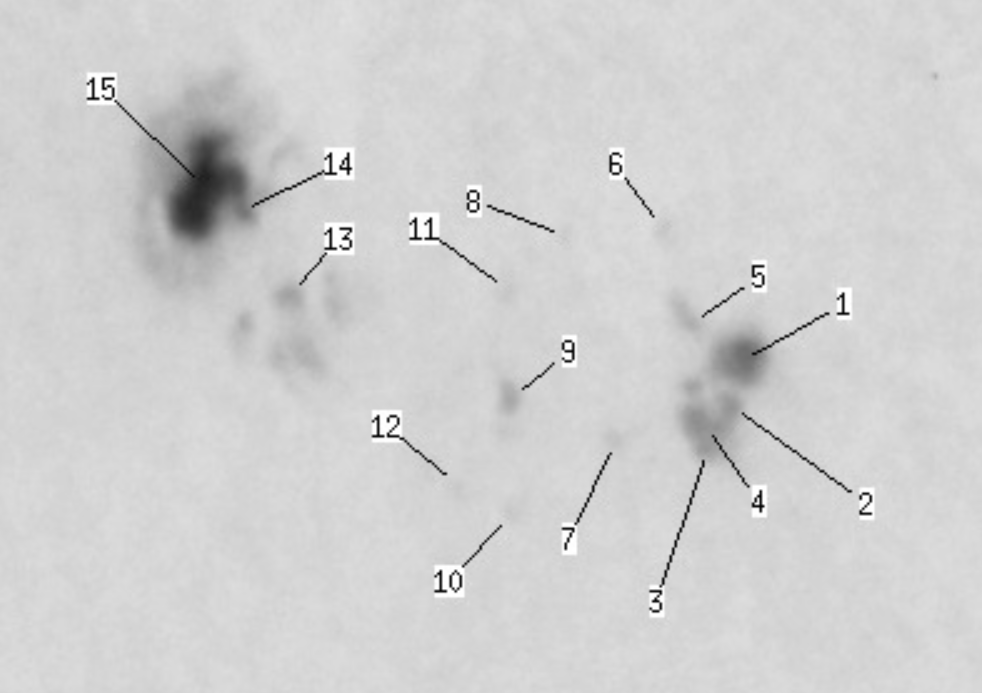
\includegraphics[width=\textwidth]{./pictures/sunspot-annotation}
    \caption{Annotated group of sunspots.}
    \label{fig:sunspot-annotation}
\end{figure}
The identification of each one of these variables carries its own challenges. In Figure~\ref{fig:sunspot-annotation} the reader can appreciate a manual annotation of a group of sunspots by an expert scientist. Each label refers to a single sunspot so the total number of sunspots in the image is equal to the number of labels that are present. Note that the annotation is not as straightforward as it seems, for example label \text{13} refers to more than one dark area while labels \textit{2, 3, 4} all map to a single black spot. We won't go into detail about why labels have been assigned this way but the reader can assume that the expert annotator has a deep understanding of the behaviour of the magnetic field and therefore he is able to distinguish real sunspot instances from artifacts. In the case of Figure~\ref{fig:sunspot-annotation} the sunspot group was found near the center of the disk, but there are cases where the sunspots appear much closer to the limb. In those cases the viewing angles are very high and the annotation is a lot harder, because of
perspective deformations and the limb darkening effect.\\
Once all the sunspots in the image have been annotated they can be clustered into groups. Again, in Figure~\ref{fig:annotated-mask} the reader can get an impression of what it means to find sunspot groups. If the magnetogram of the solar disk is available, it is fairly easy to detect active regions first, and then map each sunspot to the closest one. For the reasons that have been explained in Chapter~\autoref{capitolo2} it will be supposed that the magnetogram is not available. So, clustering has to be performed by inferring the magnetic link between each sunspot. Sunspot classification can be used as an aid for clustering. In fact, broadly determining the class while forming a group is important to make sure that the magnetic properties are respected. Nevertheless, when the cycle is near to the peak active regions tend to be very close to each other. This behaviour is showed in Figure~\ref{fig:annotated-mask}, where groups 11516 (grey) and 11517 (red) are almost overlapping. In such a situation separating or not the two groups is a rather subjective matter that causes inconsistecies.\\
Finally, the personal reduction coefficient is usually estimated statistically. Since sunspot counting is done on a daily basis, $K$ can be recalculated every day taking into account past observations. SILSO implements a similar procedure using a pilot station as a reference, and, for simplicity they recalculate once per month, instead of daily. \clearpage
\begin{figure}[h!]
    \centering
    \captionsetup{justification=centering}
    \begin{subfigure}[t]{0.45\textheight}
        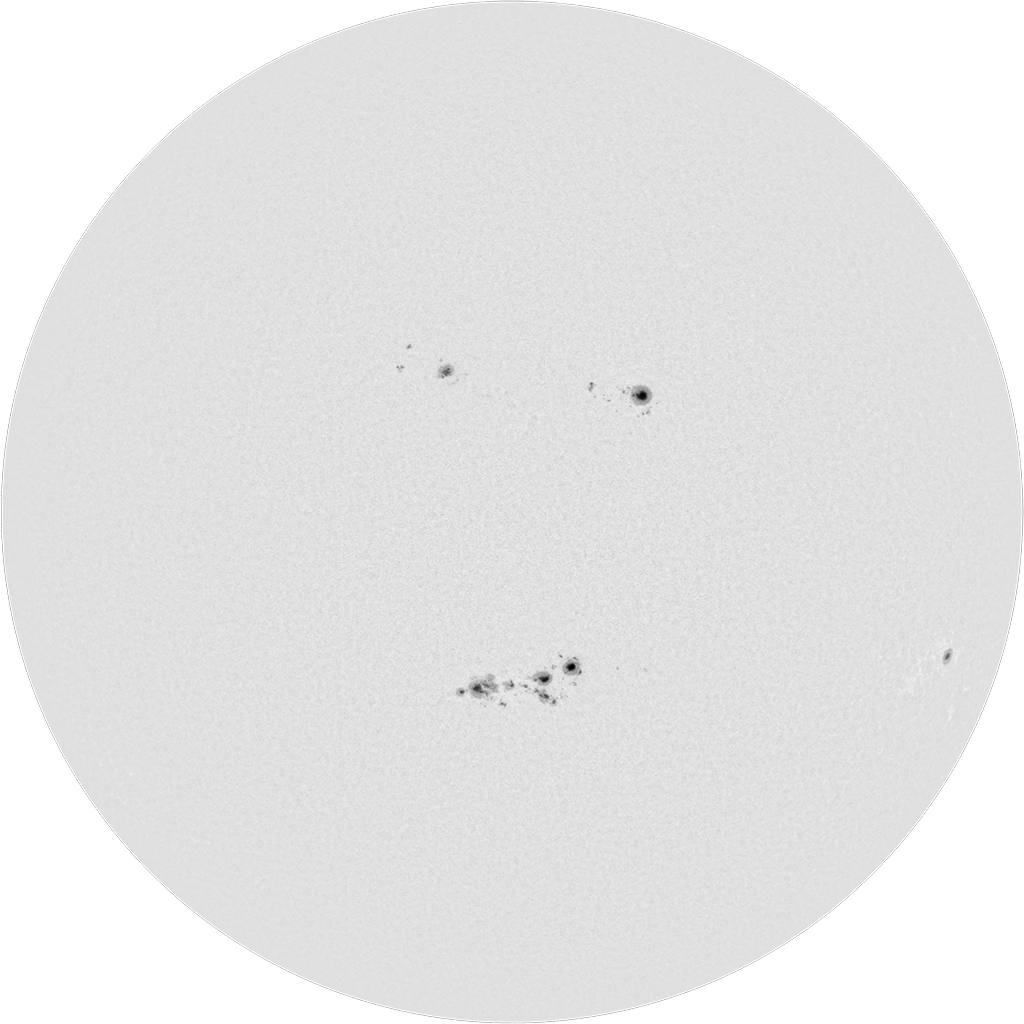
\includegraphics[width=\textwidth]{./pictures/groups-white-light}
    \end{subfigure}\vspace{3mm}
    \begin{subfigure}[t]{0.45\textheight}
        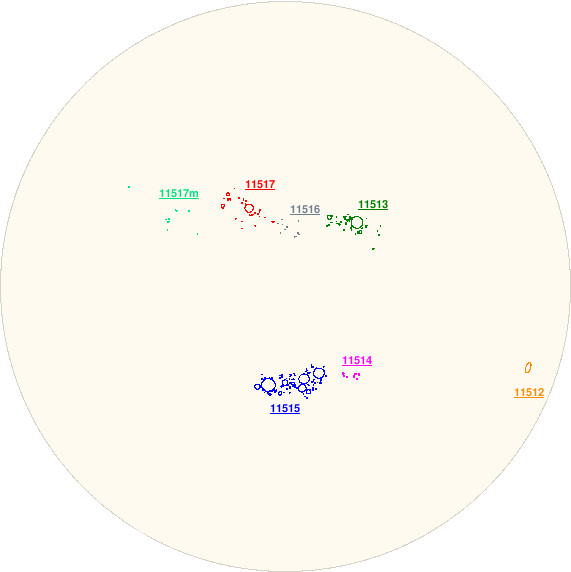
\includegraphics[width=\textwidth]{./pictures/groups-annotation}
    \end{subfigure}
    \caption{Complete solar observation, 03/07/2012. Top: full-disk white-light image, Bottom: annotated mask with colorized sunspot groups}\label{fig:annotated-mask}
\end{figure}
